\section{有限差分}
\label{sec:2.2}

有限差分是计算机求解微分方程的基本方法,这神方法的最佳特点就是它可以分析几乎
任何形态的对象、诸如大地地形或地质构造等。进行差分计算通常是一种简单的任务,其主
要问题是不稳定性。往往发生这样的现象,对一个合理的物理问题看来是合理的处理方法却
导致剧烈振荡和不收敛的计算结果。幸好,还有十分稀少的一些重要而又易于掌握的技巧可
以解决大多数不稳定性问题。

具有次要意义的一些问题是计算时间与精度问题。由于要付出更精细计算网格这样的高昂
代价方可改善精度,所以必须将计算时间与精度二者综合加以考虑。虽然选择以下几节所述方
法并非出于对猜度或计算效率的考虑,不过在这些领域内,这些方法确实是出色的。说实在的,
据我所知,某些方法完全不可能再改进了,而另一些方法改进的余地则可能很小。所谓“小”,
我的意思是指效率提高不超过五倍的改进。这样的改进很少是由于研究或试验工作的结果。
然而,鉴于它对生产工作具有重要性,进一步阅读远超出以下几节内容的文献还是很必要的。

\subsection{透镜方程}
\label{sec:2.2.1}

各种波场外推算子均可分为两部分:较复杂的部分称为绕射或偏移部分,而较简单的部
分则称作透镜部分。透镜方程引入了一个作为$x$之函数的时移,由于它正像一个光学薄透镜
在光线沿轴向投射(垂直投射)时那样起作用,故而获得透镜方程这种名称。在绕射部分
中,以某种方式隐含着对非垂直入射和透镜厚度的校正.透镜方程存在有解析解,即$\exp[i\omega t_0(x)]$
。运算时,最好是利用这种解析解而不是利用某种差分解,因为解析解没有因采用近
似计算而引起的误差。在讨论有限差分的一章中之所以会提到透镜方程,其仅有的原因完全是
由于伴随的绕射方程必须与透镜方程一起向前推进计算,所以解析解要沿很小的步长推进。

\subsection{一次导数与显式方法}
\label{sec:2.2.2}

速率为10\%的通货膨胀率$q$可用下述差分方程描述
\begin{subequations}
\begin{equation}
q_{t+1}-q_t=0.10q_t
\label{eq:2.2.1a}
\end{equation}
\begin{equation}
(1.0)q_{t+1}+(-1.1)q_t=0
\label{eq:2.2.1b}
\end{equation}
\label{eq:2.2.1}
\end{subequations}
这类一维计算可用差分系数表和数据表重新加以表示,就这一点而论,它对如何组织二维偏
微分方程的计算提供了一种范例。设有下列系数表与数据表
\begin{figure}[H]
\centering
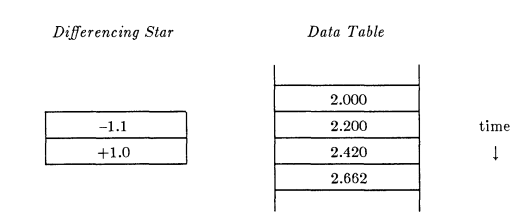
\includegraphics[width=0.5\textwidth]{new/datatable}
\caption[datatable]{差分系数表和数据表}
\label{fig:new/datatable}
\end{figure}
由于数据表中的数据满足差分方程\ref{eq:2.2.1},可将差分系数表置于数据表顶部的任何地
方。将系数表中的数乘以它下面的表中的那些数,所得互乘结果之和将为零。另一方面,如
果数据表中除一个数(初始条件)之外,所有的数都没有,则可沿时间増大方向滑动该系数
表。取互乘之和并令差分方程成立,一次计算出一个数,每一步都可解出未知数据值,从而
可将数据表中所有其余的数部填满。

当数值系数0.10周一个复数代替时,利用同一套差分系数表就要稍为繁琐一些。这种情
形下,计算结果既表现出有振荡现象,又表现出有增大和阻尼衰减的现象。

\subsection{一次导数与隐式方法}
\label{sec:2.2.3}

试以数值方法求解下述方程:
\begin{equation}
\frac{dq}{dt}=2rq
\label{eq:2.2.3}
\end{equation}
注意,在通货膨胀方程\ref{eq:2.2.1}中是$2r=.l$,那种方程是一种近似式,但是现在要注意,在
通货膨胀方程中的表达式$dq/dt$是位于时间$t+1/2$,而表达式$q$本身则位于时间$t$。没有理由
不把式\ref{eq:2.2.3}右端的$q$在时间$t$上用时间$t+1$来加以平均,因而可将整个方程均置于时间
$t+1/2$。具体说,式\ref{eq:2.2.3}的中心差分近似为
\begin{subequations}
\begin{equation}
q_{t+1}-q_t=2r\Delta t\frac{q_{t+1}+q_t}{2}
\label{eq:2.2.4a}
\end{equation}
令$\alpha=r\Delta t$,上式变为
\begin{equation}
(1-\alpha)q_{t+1}-(1+\alpha)q_t=0
\label{eq:2.2.4b}
\end{equation}
\label{eq:2.2.4}
\end{subequations}
\begin{figure}[H]
\centering
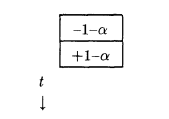
\includegraphics[width=0.25\textwidth]{new/difftable}
\caption[difftable]{差分系数表}
\label{fig:new/difftable}
\end{figure}
在固定步长的情形下,这种系数表得出的微分方程\ref{eq:2.2.3}的解比前述由通货膨胀系数表得出的解更为精确。

\subsection{显式热流方程}
\label{sec:2.2.4}

热扩散系由热流方程控制.这种方程是地震偏移方法的一个原型,15°偏移方程与该方
程形式相同,只不过热传导常数是虚数而已(偏移方程实际是Schroedinger方程,该方程
描述原子粒子扩散几率)。取$\sigma$为常数,得热流方程
\begin{equation}
\frac{\partial q}{\partial t}=\frac{\sigma}{c}\frac{\partial^2 q}{\partial x^2}
\label{eq:2.2.5}
\end{equation}
在计算机上实现式\ref{eq:2.2.5}的计算需对各偏微分作某种差分近似。最明显不过(但并非
唯一的)的办法就是采用初等微积分教程中关于微分的基本定义,就时间导数而言,这就
是
\begin{subequations}
\begin{equation}
\frac{\partial q}{\partial t}\approx \frac{q(t+\Delta t)-q(t)}{\Delta t}
\label{eq:2.2.6a}
\end{equation}
利用下标使式\ref{eq:2.2.6a}形式紧凑是很方便的
\begin{equation}
\frac{\partial q}{\partial t}\approx \frac{q_{t+1}-q_t}{\Delta t}
\label{eq:2.2.6b}
\end{equation}
\end{subequations}
在这种符号表示中,$t+\Delta t$简记为$t+1$,对于更为复杂的方程有其方便之处。取两次一阶导
数可得到二阶导数公式,由此得出$q_{t+2}-2q_{t+1}+q_t$;通常都进行时移,将该公式处理成更
为对称的形式$q_{t+1}-2q_t+q_{t-1}$。当$\Delta t$趋于零时,这两种形式是等价的,但是在$\Delta t$不为零
时,则更为对称时安排形式将更为精确。利用上标描述与$x$有关的函数,得出二阶空间导数
的有限差分近似:
\begin{equation}
\frac{\partial^2 q}{\partial x^2}\approx \frac{q^{x+1}-2q^x+q^{x-1}}{\Delta x^2}
\label{eq:2.2.7}
\end{equation}
将\ref{eq:2.2.6b}与\ref{eq:2.2.7}代入热流方程,并用符号$=$表示$\approx$,得
\begin{equation}
\frac{q_{t+1}-q_t}{\Delta t}=\frac{\sigma}{c}\frac{q_t^{x+1}-2q_t^x+q_t^{x-1}}{\Delta x^2}
\label{eq:2.2.8}
\end{equation}
令$a=\sigma \Delta t/(c\Delta x^2)$时,式\ref{eq:2.2.8}可重写为
\begin{equation}
q_{t+1}-q_t-a(q_t^{x+1}-2q_t^x+q_t^{x-1})=0
\label{eq:2.2.9}
\end{equation}
几何上,可将式\ref{eq:2.2.9}解释为$(x,t)$平面中的一种十字形系数表的计算结果,如
图\ref{fig:new/fig2-2-1}所示。在数据表内移动该十字形系数表,你会注意到,它可一次仅将一个数定位于
数据表内之未知元素位置上(即在1所指示的位置上),这就使得能从数据表顶部开始依次
计算下一行.照这样作下去,你就是在用有限差分方法求解偏微分方程。关于初始条件和边
界条件还存在其他可能的安排,诸如零斜率边界条件等。下面是一个计算机程序和验算的例
子。
\begin{figure}[H]
\centering
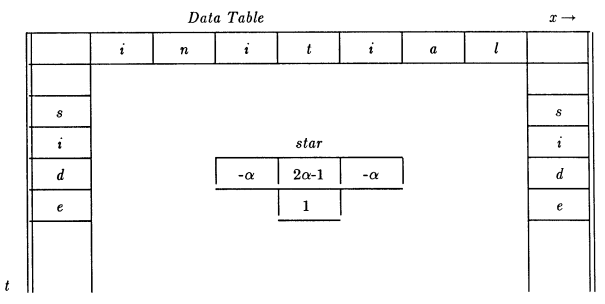
\includegraphics[width=0.95\textwidth]{new/fig2-2-1}
\caption[fig2-2-1]{一维热流方程的十字形差分系数表与数据表}
\label{fig:new/fig2-2-1}
\end{figure}
\begin{minted}{Fortran}
# Explicit heat-flow equation
real q(12),qp(12)
nx= 12

do ia== 1,2 { # stable and unstable cases

alpha = ia* . 3333 ; write(6, '(/"alpha=",f4.2)')alpha

do ix= 1,6; q(ix) = 0. # Initial temperature step
do ix=7,12; q(ix) = l.
do it= 1,6 {

write(6 , '(20f5.2)') (q(ix),ix=1,nx)
do ix=2,nx-l
qp(ix) = q(ix) + alpha* (q(ix-1)-2. * q(ix)+q(ix+1))
qp(1) = qp(2);
qp(nx)=qp(nx- 1)
do ix = 1 ,nx
q(ix) = qp(ix)
}
}
stop;end

alpha=.33
0.00 0.00 0.00 0.00 0.00 0.00 1.00 1.00 1.00 1.00 1.00 1.00
0.00 0.00 0.00 0.00 0.00 0.33 0.67 1.00 1.00 1.00 1.00 1.00
0.00 0.00 0.00 0.00 0.11 0.33 0.67 0.89 1.00 1.00 1.00 1.00
0.00 0.00 0.00 0.04 0.15 0.37 0.63 0.85 0.96 1.00 1.00 1.00
0.00 0.00 0.01 0.06 0.19 0.38 0.62 0.81 0.94 0.99 1.00 1.00
0.00 0.00 0.02 0.09 0.21 0.40 0.60 0.79 0.91 0.99 1.00 1.00

alpha=.67
0.00 0.00 0.00 0.00 0.00 0.00 1.00 1.00 1.00 1.00 1.00 1.00
0.00 0.00 0.00 0.00 0.00 0.67 0.33 1.00 1.00 1.00 1.00 1.00
0.00 0.00 0.00 0.00 0.44 0.00 1.00 0.56 1.00 1.00 1.00 1.00
0.00 0.00 0.00 0.30 -.15 0.96 0.04 1.15 0.70 1.00 1.00 1.00
0.00 0.00 0.20 -.20 0.89 -.39 1.39 0.11 1.20 0.80 1.00 1.00
0.13 0.13 -.20 0.79 -.69 1.65 -.65 1.69 0.21 1.20 0.87 0.87
\end{minted}

\subsection{鞋跃式方法}
\label{sec:2.2.5}

采用上面给出程序的困难在于,它并非对所有可能的$\alpha$数值均有效。可以看出,当$\alpha$值过
大时(亦即$\Delta x$过小时),在数据表内部区域的解包含有不断增大的振荡。出现这种现象是因
为解的低频部分还能凑合,可是高频部分却发散。出现发散现象的准确原因将是2.8节内所
进行的某些数学分析的主题。在波长长度可与或汾相比较时,差分近似因温度之不规则
性被平滑而可望与真正的热流方程一致。在短波长时,剧烈的振荡表明差分方程可以按一种
几乎与该偏微分方程完全相反的方式来行事。短波长之所以出现偏差,是因为差分算子仅在
长波长时才等于微分算子。解的发散性是一个致命问题,因为随后出现的舍入误差往往还
会破坏低频部分。

由于假设不稳定性是因时间导数位于一个与$x$方向二阶导数所在时间$t$稍微不同的时间
$t+1/2$上所引起,于是导致所谓蛙跃式方法,这种方法将时间导数取为$t-1$与$t+1$之间的差
分:
\begin{equation}
\frac{\partial q}{\partial t}\approx \frac{q_{t+1}-q_{t-1}}{2\Delta t}
\label{eq:ex2.2.10}
\end{equation}
所得蛙跃式十宇形差分系数表形式如下:
\begin{figure}[H]
\centering
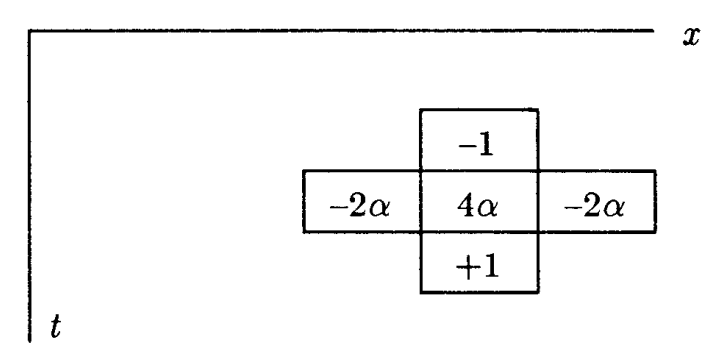
\includegraphics[width=0.5\textwidth]{new/fig-leapfrog-1}
\caption[fig-leapforg-1]{蛙跃式十宇形差分系数表形式}
\label{fig:new/fig-leapfrog-1}
\end{figure}
其实采取这种方法所得结果并不好。以后的分析将证明,对$\alpha$的所有实数值,现在的解是发
散的。将两种导数均置于相同时间位置虽然是个好主意,可是横跨许多网格点来表示一个一
阶导数,终究是个坏主意。扩展了的算子在时间方面有两个解,而不是仅只有熟知的那一个
解。数值解是两个理论解之和,不幸的是,其中一个解对$\alpha$的所有实数值是振荡增长的。

为避免所有上述这些问题(也为得到更精确的答案),我们现要转而讨论稍微更复杂一
些的求解方法,即所谓隐式方法。

\subsection{Crank-Nicolson 方法}
\label{sec:2.2.6}

Crank-Nicolson法既求得准确又可解决稳定性问题。

热流方程\ref{eq:2.2.8}曾表示为
\begin{equation*}
q_{t+1}^x-q_t^x=a[q_t^{x+1}-2q_t^{x}+q_t^{x-1}]
\end{equation*}
现在,不是整个在时间$t$上表示上述右端项,而是在$t$与$t+1$上把它平均,得出
\begin{equation}
q_{t+1}^x-q_t^x=\frac{a}{2}[(q_t^{x+1}-2q_t^{x}+q_t^{x-1})+(q_{t+1}^{x+1}-2q_{t+1}^{x}+q_{t+1}^{x-1})]
\label{eq:ex2.2.12a}
\end{equation}
此式称为Crank-Nicolson法。令$\alpha=a/2$,则差分系数为
\begin{figure}[H]
\centering
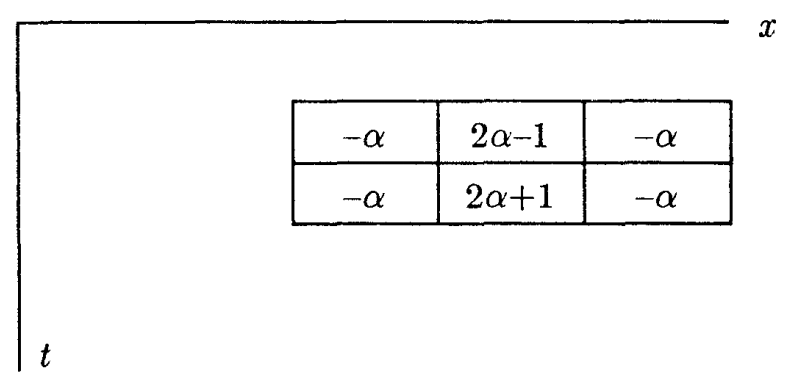
\includegraphics[width=0.5\textwidth]{new/fig-cn-1}
\caption[fig-cn-1]{蛙跃式十宇形差分系数表形式}
\label{fig:new/fig-cn-1}
\end{figure}
当把这个系数表置于数据表上时,要注意一个时间上有三个元素是未知数。为将方程也依此
处理,把式\ref{eq:ex2.2.12a}中所有的$t+1$项移至左端,而所有$t$项移至右端,得
\begin{subequations}
\begin{equation}
-\alpha q_{t+1}^{x+1}+(1+2\alpha)q_{t+1}^x-\alpha q_{t+1}^{x-1}=\alpha q_t^{x+1}+(1-2\alpha)q_t^x+\alpha q_t^{x-1}
\label{eq:2.2.13a}
\end{equation}
将所有属于$t+1$的项取为未知数,而属于$t$的项取为已知项,所以式\ref{eq:2.2.13a}的右端是已
知的,例如令其为$d_t^x$,而左端则是未知数$q_{t+1}$的一组联立方程。换言之,式\ref{eq:2.2.13a}并
未以显式的形式为我们给出每个$q_{t+1}^x$,它们是隐式地以联立方程的解给出的。如果$x$轴上只
限取五个点,则这些联立方程即为
\begin{equation}
\begin{bmatrix}
e_{lf}&-\alpha&0&0&0\\
-\alpha&1+2\alpha&-\alpha&0&0\\
0&-\alpha&1+2\alpha&-\alpha&0\\
0&0&0&-\alpha&e_{rt}
\end{bmatrix}
\begin{bmatrix}
q_{t+1}^1\\q_{t+1}^2\\q_{t+1}^3\\
q_{t+1}^4\\q_{t+1}^5
\end{bmatrix}
=
\begin{bmatrix}
d_t^1\\d_t^2\\d_t^3\\d_t^4\\d_t^5
\end{bmatrix}
\label{eq:2.2.13b}
\end{equation}
\end{subequations}
值$e_{lf}$和$e_{rt}$是可调节的,并且必须按旁侧边界条件来调节。值得注意的重要事情是,该矩阵
是三对角线矩阵,即,除三个中心对角线上的元素外,矩阵\ref{eq:2.2.13b}中所有其他元素均
为零。能够快速地得出这一类联立方程的解,其计算时间大约仅二倍于式\ref{eq:2.2.9}给出的显
式方法。事实上,由于式\ref{eq:2.2.13a}的精度高于式\ref{eq:2.2.9},允许利用非常大的时间步长$\Delta t$,
结果这种隐式方法证明是种节省时间的方法。下面给出一个可以说明即使是对很大$\Delta t$,
该方法也具有稳定性的程序。

\begin{minted}{Fortran}
# Implicit heat-flow equatioil
real q(12),d(12),e(12),f(12)

nx= 12;a=8.; write(6,'(/"a= ",f4.2)')a; alpha= .5*a
do ix= 1,6; q(ix)= 0. # Initial temperature step
do ix=7,12; q(ix)= 1.
do it== 1,4 {
write(6,'(20f5.2)') (q(ix),ix= 1,nx)
d(l)=0.; d(nx)= 0.
do ix=2,nx-l
d(ix)=q(ix) + alpha*(q(ix-l)-2.*q(ix) + q(ix+ 1))
call rtris(nx,alpha,-alpha,( l. + 2.*alpha),-alpha,alpha,d,q,e,f)
}
stop; end
# real tridiagonal equation solver

subroutine rtris(n,endl,a,b,c,endr,d,q,e,f)
real q(n),d(n),f(n),e(n)
e(1) =-a/endl; f(1) = d(1)/endl
do i = 2,n-l {
den = b + c*e(i-1); e(i) = -a/den;  f(i)= (d(i)-c*f(i-1))/den }
q(n) = (d(n)-c*f(n-1))/(endr+ c*e(n-1))
do i = n-1,1,-1
q(i) = e(i)*q(i + 1) + f(i)
return; end

a = 8.00
0.00 0.00 0.00 0.00 0.00 0.00 1.00 1.00 1.00 1.00 1.00 1.00
0.17 0.17 0.21 0.30 0.47 0.76 0.24 0.53 0.70 0.79 0.83 0.83
0.40 0.40 0.42 0.43 0.40 0.24 0.76 0.60 0.57 0.58 0.60 0.60
0.44 0.44 0.44 0.44 0.48 0.68 0.32 0.52 0.56 0.56 0.56 0.56
\end{minted}
计算中采用了求解三对角线联立方程的子程序,下一节将对该子程序加以解释。

\subsection{求解三对角线联立方程}
\label{sec:2.2.7}

全世界有很多计算力量都忙于应付求解三对角线联立方程。为参考和完整起见,本节内
容也将涉及算法。

设将联立方程写成某种差分方程组
\begin{equation}
a_iq_{i+1}+b_iq_i+c_iq_{i-1}=d_i
\label{eq.ex2.2.14}
\end{equation}
按照某种方程
\begin{equation}
q_i=e_iq_{i+1}+f_i
\label{eq.ex2.2.15}
\end{equation}
引入两个新未知数$e_i$与$f_i$,用经过时移的下标写出式\ref{eq.ex2.2.15}
\begin{equation}
q_{i-1}=e_{i-1}q_{i}+f_{i-1}
\label{eq.ex2.2.16}
\end{equation}
将\ref{eq.ex2.2.16}代入\ref{eq.ex2.2.14},得
\begin{equation}
a_iq_{i+1}+b_iq_i+c_i(e_{i-1}q_{i}+f_{i-1})=d_i
\label{eq.ex2.2.17}
\end{equation}
现将式\ref{eq.ex2.2.17}重新排列,使之类似于\ref{eq.ex2.2.15}
\begin{equation}
q_i=\frac{-a_i}{b_i+c_ie_{i-1}}q_{i+1}+\frac{d_i-c_if_{i-1}}{b_i+c_ie_{i-1}}
\label{eq.ex2.2.18}
\end{equation}
将式\ref{eq.ex2.2.18}与式\ref{eq.ex2.2.15}比较即可看出,新的未知数$e_i$与$f_i$的递归公式为
\begin{subequations}
\begin{equation}
e_i=\frac{-a_i}{b_i+c_ie_{i-1}}
\label{eq:ex2.2.19a}
\end{equation}
\begin{equation}
f_i=\frac{d_i-c_if_{i-1}}{b_i+c_ie_{i-1}}
\label{eq:ex2.2.19b}
\end{equation}
\label{eq:ex2.2.19}
\end{subequations}
首先必须给出左侧边界的某种边界条件,这种条件也许会涉及一个点或两个点。最一般性的
可能的边缘终端条件是一种在$i=0$时类似于方程\ref{eq.ex2.2.15}
的线性关系,即$q_0=e_0q_1+f_0$。
因此边界条件必须给出$e_0$与$f_0$,利用$e_0$以及所有的$a_i$,$b_i$,$c_i$,我们就可采用式\ref{eq:ex2.2.19a}
计算出所有的$e_i$。
在右端的边界,我们需要另一种边界条件,最一般性的两点式边界条件为
\begin{equation}
c_{n-1}q_{n-1}+e_{rt}q_n=d_n
\label{eq:ex2.2.20}
\end{equation}
作为特殊情形,此式包括了零值边界条件与零斜率边界条件。式\ref{eq:ex2.2.20}可与式\ref{eq.ex2.2.16}在其端点上时的情形相比
\begin{equation}
q_{n-1}=e_{n-1}q_n+f_{n-1}
\label{eq:ex2.2.21}
\end{equation}
$q_n$与$q_{n-1}$均为未知数,不过,式\ref{eq:ex2.2.20}与\ref{eq:ex2.2.21}是两个方程,所以求解很容易。最
后一步是取$q_n$的值,并在式\ref{eq.ex2.2.16}中利用它计算出$q_{n-1}$、$q_{n-2}$、$q_{n-3}$等等。

如果你希望尽可能充分发挥你的讨算机潜力,则应注意有关这种算法的若干事实:
\begin{enumerate}
\item $e_i$值的计算通过$a_i$、$b_i$、$c_i$而与介质有关,但与解$q_i$无关(即使是通过$d_i$),这意昧着它有
可能节省计算时间,而可重复利用$e_i$。
\item 许多计算机都是除法比乘法慢得多,因此,可以将式\ref{eq:ex2.2.19a}、\ref{eq:ex2.2.19b}中的除数之倒数一次求出来,而且或许可存储起来以备重复使用。
\end{enumerate}
\subsection{导数$\partial^3/\partial x^2\partial z$}
45°绕射方程不同于15°绕射方程之处在于前者包括有导数$\partial^3/\partial x^2\partial z$。幸运的是,这种导
数可适应六点差分系数表
\begin{figure}[H]
\centering
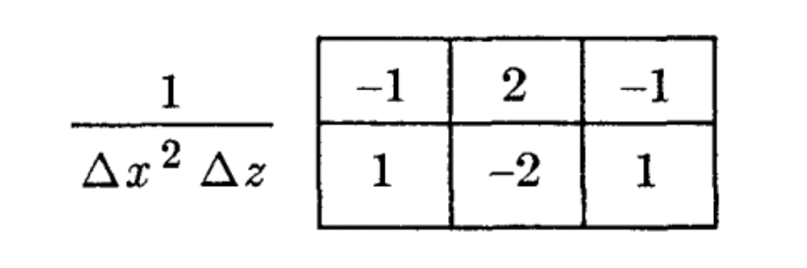
\includegraphics[width=0.5\textwidth]{new/fig-2-2-22}
\caption[fig-2-2-22]{六点差分系数表形式}
\label{fig:new/fig-2-2-22}
\end{figure}
所以,除了改变系数表上的六个系数之外,它并不会对计算效率造成什么影响。

\subsection{高维方程的困难}
\label{sec:2.2.8}

迄今,为获得节省时间而又精确可靠的求解偏微分方程之差分方法,我们还未遇到麻
烦,隐式方法已可满足所有的需要。
可是,在高于一维的空间域,隐式方法的运算时间就高
得使人不敢问津了。我们将以$\partial^2/\partial x^2$推广为$\partial^2/\partial x^2+\partial^2/\partial y^2$的普通问题为例来讨论一下其
理由何在。最简单的情形就是热流方程,由Crank-Nicolson方法给出式\ref{eq:2.2.13a}。引入缩
写$\delta_{xx}q=q^{x+1}-2q^x+q^{x-1}$,式\ref{eq:2.2.13a}变为
\begin{equation}
(1-\alpha\delta_{xx})Q_{t+1}=(1+\alpha\delta_{xx})Q_{t}
\label{eq:ex2.2.23}
\end{equation}
左端括内的表达式代表一个三对角线矩阵,关键之处在于4求解未知数$Q_{t+1}$向量的三对角
线联立方稆。值把庆幸的是有一种获得该解的特殊算法,其计算时间仅随矩阵之大小而线性
增加。现在就从$x$的一维物理空间转而讨论二维空间$(x,y)$,
令$\alpha$表示式\ref{eq:ex2.2.23}中的
数值常数,于是按时间步进的方程为
\begin{equation}
[1-\alpha(\delta_{xx}+\delta_{yy})]Q_{t+1}=[1+\alpha(\delta_{xx}+\delta_{yy})]Q_t
\label{eq:ex2.2.24}
\end{equation}
未知数$Q_{t+1}$是$x$与$y$的二维函数,可用一个矩阵表示。其次,我们将解释一下左端括号内的
表达式,结果证明它是一个四维矩阵!

为搞清楚这个矩阵的意义,将利用从二维投影为一维映像的办法来加以阐述。设温度Q
定义于$4\times 4$格点上,将网格各点进行编号的一种很自然的方式为
\begin{equation}
\begin{bmatrix}
11&12&13&14\\
21&22&23&24\\
31&32&33&34\\
41&42&43&44
\end{bmatrix}
\label{eq:ex2.2.25}
\end{equation}
就代数运算目的而言,这十六个数可投影为一个向量,有许多方法可作到这点。简单方法是
利用下面的按列排列的方式将式\ref{eq:ex2.2.25}中的各位置同列向量分量联系起来:
\begin{equation}
\begin{bmatrix}
1&5&9&13\\
2&6&10&14\\
3&7&11&15\\
4&8&12&16
\end{bmatrix}
\label{eq:ex2.2.26}
\end{equation}
二阶差分算子具有下列$(x,y)$平面内的十字形系数表
\begin{figure}[H]
\centering
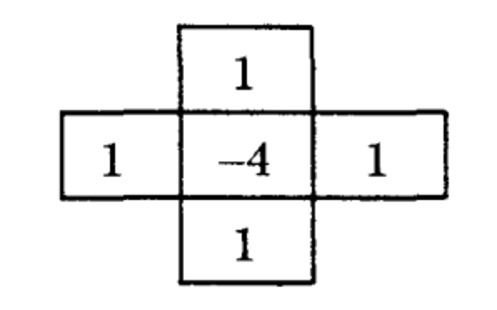
\includegraphics[width=0.35\textwidth]{new/fig-2-2-27}
\caption[fig-2-2-27]{十字形系数表}
\label{fig:new/fig-2-2-27}
\end{figure}
将此十字形系数置于式\ref{eq:ex2.2.26}所在$(x,y)$平面内并沿其周围移动。可惜,由于仅
有十六个点,你看到的有许多是以边缘和端点为主。试使中心系数$-4$覆盖十六个点中的一
个,对该矩阵的每一个位置均如此作,系数1是否离开了端点别去管它。开始时,令式\ref{fig:new/fig-2-2-27}
中的系数$-4$覆盖在式\ref{eq:ex2.2.26}的左上角之1的位置上,此时可观察到系数表中有两个
1位于该矩阵的2和5上。将1填入表\ref{fig:new/fig-2-2-1}中的2的位置,此时可看到有三个1分别位于1、3、6的位置。
将这些1填入表\ref{fig:new/fig-2-2-1}所示系数矩阵的第二行的各相应列的位置。然后再将$-4$置于3的位置,此时表
有三个1分别位于2、4、7的位置......,如此继续做下去,直至得到$16\times 16$方阵如表\ref{fig:new/fig-2-2-1}所示。
\begin{figure}[H]
\centering
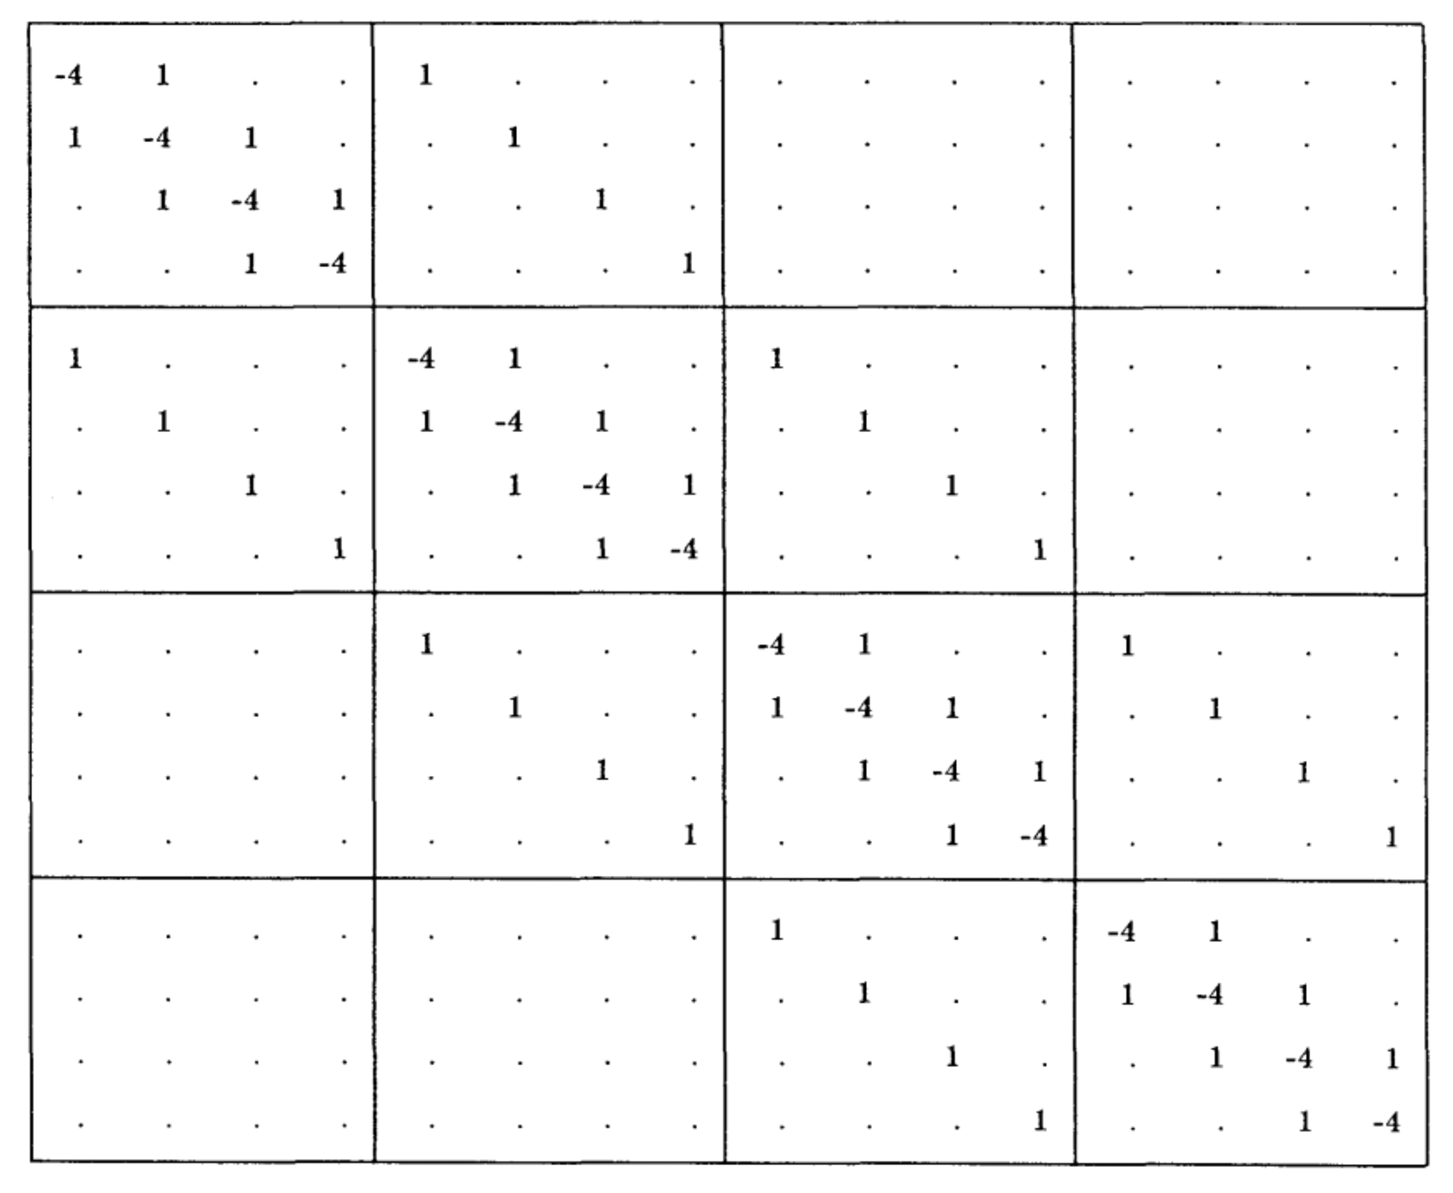
\includegraphics[width=0.85\textwidth]{new/fig-2-2-1}
\caption[fig-2-2-1]{Laplace算子的二维系数矩阵}
\label{fig:new/fig-2-2-1}
\end{figure}
现在,拉氏二维系数矩阵已经构成,我们可转而解释方程\ref{eq:ex2.2.24}的意义了。未知数
$Q_{t+1}$矩阵已投影为一个十六点的列向量,因而括号内的表达式乘上$Q_{t+1}$就可投影为$16\times 16$
矩阵。显然,表\ref{fig:new/fig-2-2-1}中每一包含点号之处均为该二维系数矩阵的零元素所在之处。矩阵含
有许多零元素似乎是幸运的,这使我们有希望得出联立方程快速解法,可惜的是,尽管经过
努力,还从没找到过一好较好的方法看来得要求计算量与$N_3$成比例,在所述情形
下,$N = 4$。根据我们对一维问题的经验,我们
当中那些曾经搞过这种问题的人们期待有一
种与$N_2$成比例的方法,这是显式方法的计算量——
实质上就是计算式\ref{eq.ex2.2.16}右端的计算
量。即使采用隐式方法的所有特点也证明不了与$N$成比例的计算量是可能的。其次较好的方
法足分离法。

\subsection{习 题}
\label{sec:2.2.9}

\begin{enumerate}

\item 在固定$\omega$情形下试以式\ref{eq:ex2.2.12a}的形式写出$(x,z)$空间内的45°绕射方程。

\item 在固定$\omega$情形下试以式\ref{eq:ex2.2.12a}的形式写出$(x,z)$空间内的45°绕射方程。

\item 试解释利率为虚数$i/10$时的通货膨胀方程。
\end{enumerate}
